\documentclass[12pt]{report}
\usepackage[utf8]{inputenc}
\usepackage{amsmath}
\usepackage{indentfirst}
\usepackage{graphicx}
\usepackage{svg}
\graphicspath{ {images/} }
\usepackage{caption}
\usepackage{subcaption}
\usepackage[a4paper,width=150mm,top=25mm,bottom=25mm,bindingoffset=6mm]{geometry}
\usepackage{fancyhdr}
\pagestyle{fancy}
\fancyhead{}
\fancyhead[RO,LE]{CosmOS real-time operating system whitepaper}
\fancyfoot{}
\fancyfoot[LE,RO]{\thepage}
\fancyfoot[CO,RE]{}
\renewcommand{\headrulewidth}{0.4pt}
\renewcommand{\footrulewidth}{0.4pt}
\newcommand{\inlinecode}{\texttt}
\usepackage{tikz}
\usetikzlibrary{fit, positioning}
\usepackage{hyperref}
\bibliographystyle{ieeetr}
\usepackage{biblatex}
\usepackage{lipsum}
\usepackage{mathrsfs}
\usepackage{float}
\usepackage{bm}
\usepackage{amsfonts}
\usepackage{lipsum}
\usepackage{etoolbox}
\usepackage{titlesec}
\usepackage{comment}
\usepackage{listings}
\usepackage[acronym]{glossaries}
\usepackage[withpage, printonlyused]{acronym}
\usepackage{datetime}
\usepackage{caption}

\newdateformat{monthdayyeardate}{%
  \monthname[\THEMONTH]~\THEDAY, \THEYEAR}

\makeatletter
\g@addto@macro\caption@prepareslc{%
  \let\acused\@gobble
  \let\AC@placelabel\@gobble}
\makeatother

\definecolor{mygreen}{rgb}{0,0.6,0}
\definecolor{mygray}{rgb}{0.5,0.5,0.5}
\definecolor{mymauve}{rgb}{0.58,0,0.82}

\lstset{ %
  backgroundcolor=\color{white},   % choose the background color
  basicstyle=\footnotesize,        % size of fonts used for the code
  breaklines=true,                 % automatic line breaking only at whitespace
  captionpos=b,                    % sets the caption-position to bottom
  commentstyle=\color{mygreen},    % comment style
  escapeinside={\%*}{*)},          % if you want to add LaTeX within your code
  keywordstyle=\color{blue},       % keyword style
  stringstyle=\color{mymauve},     % string literal style
  showstringspaces=false
}

\makeatletter
\patchcmd{\chapter}{\if@openright\cleardoublepage\else\clearpage\fi}%
    {\par\addvspace{\baselineskip}}{}{}
\titlespacing*{\chapter}{0mm}{3em}{1em}
\patchcmd{\ttl@save@mkschap}{*}{}{}{}
\makeatother

\titleformat{\chapter}[display]
  {\normalfont\bfseries}{}{0pt}{\Huge}

\setcounter{tocdepth}{4}
\setcounter{secnumdepth}{5}

\definecolor{CosmosBlue}{RGB}{0,74,173}

\hypersetup
{
    colorlinks=true,
    linkcolor=black,
    urlcolor=CosmosBlue,
}

\urlstyle{same}

\begin{document}
\parindent=0.5cm

\begin{titlepage}
    \begin{center}
 
        \begin{figure}[H]
		\begin{center}
		
\includegraphics[width=0.5\textwidth]{images/cosmosWhite.png}
		\end{center}
		\end{figure}
		
		\rule{9.8cm}{0.4pt}\\
        \Large
        \textbf{IDEAS BEHIND COSMOS} \\
        
        \vspace{0.25cm}
        
  		\normalsize
        CosmOS real-time operating system whitepaper\\
        \rule{9.8cm}{0.4pt}
        \vspace{1cm}        
        
        \textbf{PAVOL KOSTOLANSKY and FLORIAN LASCHOBER}\\
        
        
        \vspace*{\fill}
        \normalsize
        
        \monthdayyeardate\today
        
    \end{center}


    
\end{titlepage}

\newpage

\vspace*{-2.5cm}
\tableofcontents

\cleardoublepage
\phantomsection
\addcontentsline{toc}{chapter}{Acronyms}
\vspace*{-2.5cm}
\chapter*{Acronyms}
\begin{acronym}[]
\acro{API}{Application Programming Interface}
\acro{CIL}{CosmOS Integration Layer}
\acro{CPU}{Central Processing Unit}
\acro{GUI}{Graphical User Interface}
\acro{ISR}{Interrupt Service Routine}
\acro{JSON}{JavaScript Object Notation}
\acro{MCU}{Micro-Controller Unit}
\acro{OS}{Operating System}
\acro{UI}{User Interface}
\acro{WCET}{Worst-Case Execution Time}
\end{acronym}

\cleardoublepage
\phantomsection
\addcontentsline{toc}{chapter}{\listfigurename}
\vspace*{-2.5cm}
\listoffigures

\cleardoublepage
\phantomsection
\addcontentsline{toc}{chapter}{\listtablename}
\vspace*{-2.5cm}
\listoftables

\newpage

\vspace*{-2.5cm}
\chapter{Introduction}
\section{Motivation}
\indent CosmOS is an open-source project that we have initiated since 2020. We aim to create a hybrid operating system that offers performance and safety features within one system.\\
\indent The CosmOS architecture also allows the generation of all configuration code by model descriptions to increase productivity, make code portable, and enforce consistency. We created a set of tools with a graphical user interface to help users with the CosmOS deployment, consisting of configuration, validation, and code generation. \\
\indent It also supports the C/C++ language with the dynamic allocation and allows users to develop more complex algorithms. \\
\indent We developed CosmOS according to safety-critical design principles and coding best practices and we will strive to enhance the overall quality and safety of the software for the future releases.

\section{Architecture}
\indent CosmOS architecture is microkernel-based and implements a near-minimum amount of the operating system’s software.\\ 
\indent The main parts of the CosmOS microkernel is scheduling, memory handling, and data exchange interface. Data exchange interface is the operating system basic inter-program communication model. The microkernel can be easily expanded either with system jobs if it is necessary and make the microkernel modular, even though is highly suggested to implement all services in the user space and use data exchange interface for the inter-program communication as it is shown in the figure \ref{fig:systemArchitecture}.\\
\indent The programs are running in the user space and each of them is encapsulates its threads and tasks, providing them a safe memory space for the data, and heap for the dynamic allocation. This design allows users to implement programs with multiple safety levels without any interference between them. \\
\indent To ensure memory safety, the operating system configuration is completely static that includes also configured programs, tasks and threads and remain constant during the run-time. 
\begin{figure}[H]
\begin{center}
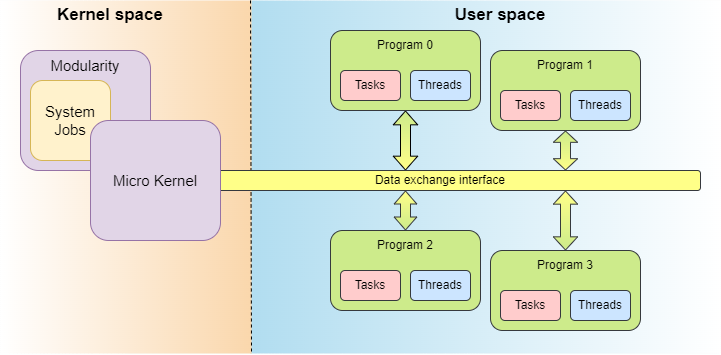
\includegraphics[width=1\textwidth]{images/system_architecture.png}
\caption{System architecture simplified diagram}
\label{fig:systemArchitecture}
\end{center}
\end{figure}

\section{Software layers}
CosmOS is composed of three main software layers:
\begin{itemize}
\vspace{-0.2cm}\item The application layer contains the user code.
\vspace{-0.2cm}\item The core layer contains kernel modules and their configuration without any microcontroller or compiler dependencies. It comprises the configuration (generated) units and non-generated units.
\vspace{-0.2cm}\item The integration layer contains units providing \ac{API} for the core layer, and it is microcontroller-specific.
\end{itemize}


\section{Main features}
We implemented multiple safety concepts to ensure it offers safety and performance features.\\
\indent The following list contains the main features of the CosmOS and CustomBox:
\begin{itemize}
\vspace{-0.2cm}\item The CustomBox \ac{GUI} helps users with configuration, generation and deployment.
\vspace{-0.2cm}\item Support for multi-core microcontrollers.
\vspace{-0.2cm}\item Hybrid scheduling combines the cyclic real-time non-preemptive scheduling and the multi-threading preemptive scheduling.
\vspace{-0.2cm}\item Memory mapping and memory protection of tasks/threads stacks, user program heaps, and user program data.
\vspace{-0.2cm}\item Memory manager supports thread-safe dynamic allocations.
\vspace{-0.2cm}\item Inter-program safe data transfers.
\vspace{-0.2cm}\item Configurable tasks/threads permissions for data transfers.
\vspace{-0.2cm}\item Possibility to implement drivers in application layer with configurable peripheral access.
\vspace{-0.2cm}\item Modular kernel expansion by system jobs with inner scheduling.
\vspace{-0.2cm}\item Configurable synchronization primitives.
\vspace{-0.2cm}\item Highly portable and modular design, which is easy to port and expand.
\end{itemize}


\section{Workflow}
In the figure \ref{fig:systemArchitecture} is shown the workflow diagram of the CosmOS. CustomBox tool helps with most of the configuration steps.\\
\indent First, user has to choose and download the integration and core bundle. These bundles contains all necessary non-generated source code.\\
\indent Later user configures the operating system modules and creates the programs, tasks and threads. After the configuration is completed, user can generate the configuration source code. \\
\indent The last step is to implement user code, compile and flash the board.

\begin{figure}[H]
\begin{center}
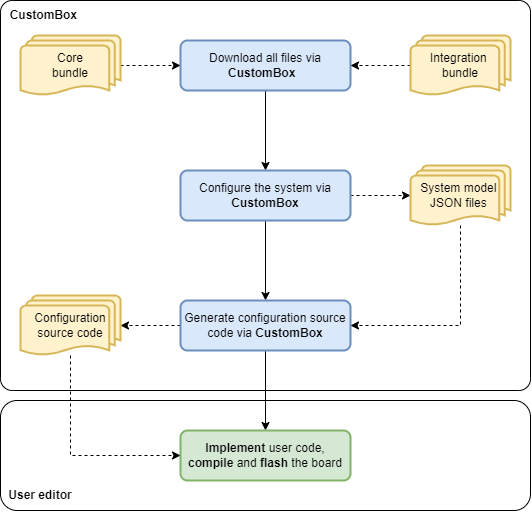
\includegraphics[width=0.9\textwidth]{images/workflow.png}
\caption{CosmOS workflow diagram}
\label{fig:workflow}
\end{center}
\end{figure}



\newpage

\vspace*{-2.5cm}
\chapter{Technical solutions}
\section{Core layer}
We designed the core layer with a focus on the minimal compiler and microcontroller dependencies. A set of required \ac{API} was created to interface with peripherals and must be implemented during the microcontroller integration process in the \ac{CIL}. \\
\indent The core layer contains multiple kernel and support modules, such as operating system run-time specific dynamic allocation implementations, which consist of smaller parts called units. With this structure, we can test all units separately with unit tests. We will talk about the each module technical details later in this chapter.\\
\indent To interface with core layer from the application layer, a generated Cosmos \ac{API} and direct kernel module's \ac{API} are provided to user as it is shown in the figure \ref{fig:coreLayer}.

\begin{figure}[H]
\begin{center}
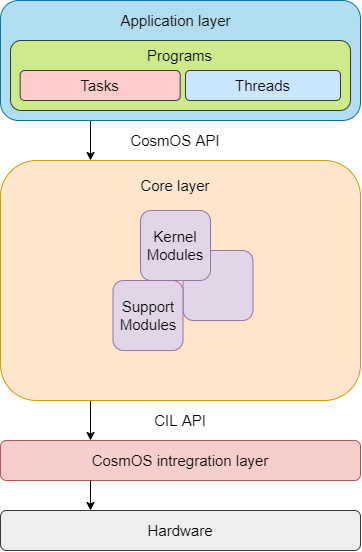
\includegraphics[width=0.5\textwidth]{images/cosmos_structure.png}
\caption{Core layer connection with application and integration layer}
\label{fig:coreLayer}
\end{center}
\end{figure}

\subsection{Types}
The CosmOS types module is divided into these smaller units:
\begin{itemize}
\vspace{-0.2cm}\item standard
\vspace{-0.2cm}\item macro
\vspace{-0.2cm}\item configuration
\vspace{-0.2cm}\item variable
\end{itemize}

\textbf{Standard} types define the state types, such as function return types or internal module states. Standard types also define the generic types used in the operating system, which are not specifically related to the configuration of modules.\\

\textbf{Macro} types are used for the macro definitions, often created to eliminate compiler dependencies to specific build-in functions by creating a generic macro with multiple macro guards for every supported compiler. These macros are static and not generated.\\

\textbf{Configuration} contains type definitions that are often used for the operating system modules configuration, specifically for the constant data. As they are constant during the runtime, they can be mapped to the CosmOS constant data section and protected by memory protection against any modifications (privileged and unprivileged). This memory section can be cached for improving performance since it contains only constant data. No cache invalidation during the runtime is needed. The configuration structures are connected its variable data via pointers, to keep the variable structure addresses protected against any modification as it is shown in figure \ref{fig:configurationVariableConnection}\\

\textbf{Variable} contains type definitions often used for the operating system modules configuration, specifically for the variable data. These types do not have to stay constant during the runtime, and they are mapped to the variable data section protected by memory protection against any unprivileged modifications. Privileged software can modify these variables. This memory section can be cached, but cache invalidation is required every time the data is changed.

\begin{figure}[H]
\begin{center}
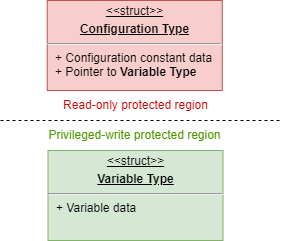
\includegraphics[width=0.5\textwidth]{images/types.png}
\caption{Configuration and variable type connection}
\label{fig:configurationVariableConnection}
\end{center}
\end{figure}

\subsection{System definitions}
The system definitions module contains a subset of system definitions units for each configurable operating system core module.\\
\indent In the C language terminologies, each of these units is only a classic header file with macro definitions, which are used in the configuration of variable types.\\
\indent The system definitions macros are visible to users and can be used in the application layer. However, we recommend that you only use CosmOS generated \ac{API} as a more error prevention method.

\subsection{Switches}\label{switchModule}
The switches module allows the user and integrator to turn on/off some of the operating system functionalities, which might depend on hardware or are just optional features and do not affect the operating system. \\
\indent This module has one switch header file per functionality that might be turned on/off during the system configuration. This header file provides switch macro \ac{API}, which can be mapped to the real function implementations or serve as stubbed functions. Therefore, we don't have to create macro guards around specific function calls.

\subsection{Stack}
The stack module is used mainly as a configuration module. It contains all necessary information about the configured stack memory sections (e.g., task/thread/kernel stacks), which are further used in multiple operating system processes. This module also provides \ac{API} for interaction with the stack module configuration structure.

\subsection{Heap}
The heap module is used mainly as a configuration module. It contains all necessary information about program heap memory sections, which are further used in multiple operating system processes, such as dynamic allocations. This module also provides \ac{API} for interaction with the heap module configuration structure.

\subsection{Schedulable}\label{schedulable}
Schedulables are the base structures that the operating system's scheduler can schedule. Task and threads structures are schedulable-based structures extending it with their specific members. This module also provides \ac{API} for interaction with the schedulable module configuration structure. The simplified diagram of the schedulable structure is shown in figure \ref{fig:schedulableStructure}.

\begin{figure}[H]
\begin{center}

\includegraphics[width=0.5\textwidth]{images/schedulable_structure.png}
\caption{Schedulable structure simplified diagram}
\label{fig:schedulableStructure}
\end{center}
\end{figure}

\subsection{Task}
Tasks are one of the two possible schedulable extensions as aforementioned. Tasks are cyclic schedulables used for the critical software execution (non-preemptive) with a strict period and configurable worst-case execution time. This allows the user to keep a tight schedule for some of the critical software running in the application layer of the operating system. Tasks can be configured in such a way that they can access some of the system resources without using kernel services. For example, they can access specific protected memory regions, such as peripherals. Tasks are configured via the CosmOS CustomBox \ac{GUI} in the tab Tasks. This module also provides \ac{API} for interaction with the task module configuration structure. The simplified diagram of the task structure is shown in figure \ref{fig:taskStructure}.

\begin{figure}[H]
\begin{center}

\includegraphics[width=0.55\textwidth]{images/task_structure.png}
\caption{Task structure simplified diagram}
\label{fig:taskStructure}
\end{center}
\end{figure}

\subsection{Thread}
Threads are one of the two possible schedulable extensions as aforementioned. Threads are used for non-critical software execution. They can be preempted and scheduled based on their unique priority (within the core they are bound to). Threads can be configured in such a way that they can access some of the system resources without using kernel services. For example, they can access specific protected memory regions, such as peripherals. Threads are configured via the CosmOS CustomBox \ac{GUI} in the tab Threads. This module also provides \ac{API} for interaction with the thread module configuration structure. The simplified diagram of the thread structure is shown in figure \ref{fig:threadStructure}.

\begin{figure}[H]
\begin{center}

\includegraphics[width=0.55\textwidth]{images/thread_structure.png}
\caption{Thread structure simplified diagram}
\label{fig:threadStructure}
\end{center}
\end{figure}

\subsection{Program}
Programs consist of tasks and threads that the user can easily assign to the desired program. This is to share program resources (such as program data and program heap) with multiple tasks and threads. Running those threads and tasks within the context of one program is described further in paragraph \ref{programMemoryProtection}. The program also has its memory section (described in detail in paragraph \ref{programMemorySection}).The user can configure the data memory and the heap memory size via the CosmOS CustomBox \ac{GUI} in the tab Programs. This module also provides \ac{API} for interaction with the program module configuration structure. The simplified diagram of the program structure is shown in figure \ref{fig:programStructure}.

\begin{figure}[H]
\begin{center}

\includegraphics[width=0.5\textwidth]{images/program_structure.png}
\caption{Program structure simplified diagram}
\label{fig:programStructure}
\end{center}
\end{figure}

\subsection{Mutex}
Mutexes are one of the synchronization primitives that are implemented in CosmOS. A mutex is designed to grant exclusive access to shared resources to the specific thread. The mutex locking mechanism can be used only for threads within one program. In CosmOS, we implemented two ways of obtaining a mutex. One way is a non-blocking method and does not cause thread preemption in case of unsuccessful locking of the mutex. In case of unsuccessful locking of the mutex, the other way will trigger the thread preemption and unblock it after the mutex is unlocked again. The mutex implementation also provides additional protection against a deadlock.

\subsection{Semaphore}
Semaphores are one of the synchronization primitives that are implemented in CosmOS. A semaphore is designed to grant exclusive access to a critical section to a specific thread. The semaphore locking mechanism can be used only for threads within the operating system instead of the mutexes, which can be only used within the program. In CosmOS, we implemented two ways of obtaining a semaphore. One way is a non-blocking method and does not cause thread preemption in case of unsuccessful locking of the semaphore. In case of unsuccessful locking of the semaphore, the other way will trigger the thread preemption and unblock it after the semaphore is unlocked again. The semaphore implementation also provides additional protection against a deadlock.

\subsection{Spinlock}
Spinlocks are one of the synchronization primitives that are implemented in CosmOS. A spinlock is designed to grant exclusive access to shared resources to a specific schedulable (task/thread). The spinlock locking mechanism can be used in tasks and threads within the operating system. In CosmOS, we implemented two ways of obtaining a spinlock. One way is the non-spinning method and does not cause spinning in the loop waiting for spinlock release in case of not successful locking of the spinlock. In case of unsuccessful locking of the spinlock, the other way will wait in a loop until the spinlock is unlocked again. The spinlock implementation also provides additional protection against a deadlock.

\subsection{Alarm}\label{alarm}
The alarm module is a necessary part of the thread sleep feature implementation in CosmOS. For each configured thread in the operating system, there is one alarm structure generated. The alarm structure contains a countdown timer, which is loaded during the sleep thread \ac{API} call and updated every time the system timer triggers the scheduler algorithm. The alarm structure also stores its state - either activated or deactivated which tells the scheduler to update only activated alarms to decrease execution time. When the alarm expires, the thread is unblocked again by setting its state to ready, and the alarm is disabled.
The simplified diagram of the alarm structure is shown in figure \ref{fig:alarmStructure}.

\begin{figure}[H]
\begin{center}

\includegraphics[width=0.5\textwidth]{images/alarm_structure.png}
\caption{Alarm structure simplified diagram}
\label{fig:alarmStructure}
\end{center}
\end{figure}

\subsection{Scheduler}
The scheduler module is dedicated to task and thread scheduling. CosmOS implements a hybrid scheduling algorithm that is driven by the system timer or specific function calls that may trigger the reschedule such as mutexes, semaphores, channels, and interrupts, in addition to the system timer and consists of two parts:
\begin{itemize}
\vspace{-0.2cm}\item classic scheduling
\vspace{-0.2cm}\item performance scheduling
\end{itemize}

Both algorithms work with the \textbf{\nameref{schedulable}} structure, which contains basic information for the scheduler. In CosmOS, we differentiate between two basic types of schedulable extension.
\begin{itemize}
\vspace{-0.2cm}\item critical task
\vspace{-0.2cm}\item non-critical thread
\end{itemize}
Both inherit the schedulable data structure and add some necessary data for the specific extension. The main difference between task and thread is shown in table \ref{tab:TaskThreadDifference}.

\begin{table}[H]
\centering
\caption{ The main difference between task and thread }
\centering
\begin{tabular}{|c|c|c|}
\hline
& \textbf{Task} & \textbf{Thread} \\
\hline \hline
It is periodic with a fixed period & \checkmark & --- \\
\hline
Can be preempted & --- &  \checkmark \\
\hline
Is killed after \ac{WCET} & \checkmark & ---\\
\hline
Stack space is reused & \checkmark & ---\\
\hline
Floating-point usage allowed & \checkmark & \checkmark \\
\hline
Can use dynamic allocation & --- & \checkmark \\
\hline
Can use spinlocks & \checkmark & \checkmark \\
\hline
Can use mutexes & --- & \checkmark \\
\hline
Can use semaphores & --- & \checkmark \\
\hline
Can use buffers (inter-program, inter-core) & \checkmark & \checkmark \\
\hline
Can use channels (inter-program, inter-core) & --- & \checkmark \\
\hline
Can handle interrupts & --- & \checkmark \\
\hline
Can be put to sleep & --- & \checkmark \\
\hline
\end{tabular}
\label{tab:TaskThreadDifference}
\end{table}

The simplified diagram of the scheduler structure is shown in figure \ref{fig:schedulerStructure}.

\begin{figure}[H]
\begin{center}

\includegraphics[width=0.55\textwidth]{images/scheduler_structure.png}
\caption{Scheduler structure simplified diagram}
\label{fig:schedulerStructure}
\end{center}
\end{figure}

\subsubsection{Classic scheduling}\label{classicScheduling}
The classic scheduling algorithm handles cyclic non-preemptive critical tasks scheduling. It uses a static schedule table generated by CustomBox. \\
\indent The main idea of the classic scheduling was to reduce the number of system timer interrupts and allow the processor to stay in some of the low power modes for a longer time.\\
\indent The main characteristics of the classic scheduling algorithm are:
\begin{itemize}
\vspace{-0.2cm}\item The algorithm uses the hyper period that is defined as the least common multiple of the tasks periods.
\vspace{-0.2cm}\item Tasks are cyclically triggered with their period.
\vspace{-0.2cm}\item Tasks use wrappers with system call that signalizes the operating system after a user code is executed.
\vspace{-0.2cm}\item If the system call is not executed before the timer interrupt occurs, the safety reaction is triggered.
\vspace{-0.2cm}\item The scheduler always sets timer ticks either to the \ac{WCET} or the next start time.
\end{itemize}
\indent In figure \ref{fig:ClassicScheduling} shows the classic scheduling diagram with naming conventions related to the reference hardware architecture.\\

\begin{figure}[H]
\begin{center}
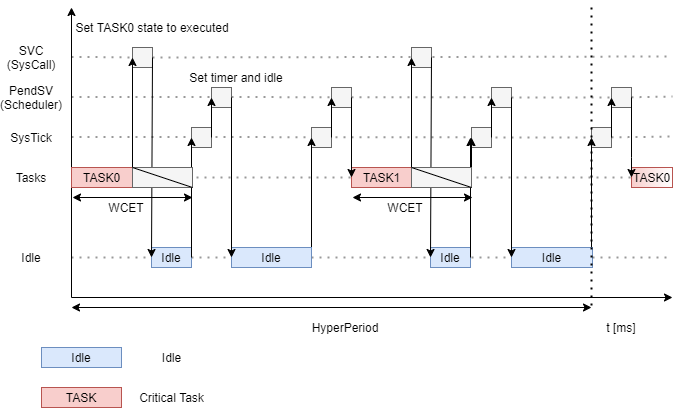
\includegraphics[width=0.9\textwidth]{images/classic_scheduling.png}
\caption{Classic scheduling diagram}
\label{fig:ClassicScheduling}
\end{center}
\end{figure}

Figure \ref{fig:SafetyReactionScheduling} shows a safety reaction to the worst critical execution time exceeding naming conventions related to the reference hardware architecture. The safety reaction is triggered directly in the system timer handler to minimize the delay.\\

\begin{figure}[H]
\begin{center}
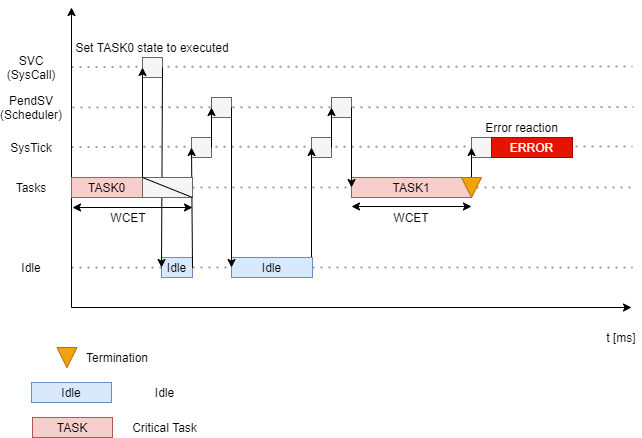
\includegraphics[width=0.9\textwidth]{images/taskWrapper.png}
\caption{Exceeding the worst critical execution time}
\label{fig:SafetyReactionScheduling}
\end{center}
\end{figure}

\subsubsection{Performance scheduling} \label{performanceSchedulingSubSubsection}
The performance scheduling algorithm handles the preemptive non-critical threads scheduling. It uses a non-critical thread queue to take the highest priority thread as fast as possible each time the rescheduling event occurs. Performance scheduling algorithm also offers to stop the thread's execution caused by multiple events, such as putting the non-critical thread to sleep, being blocked by a mutex or semaphore. \\
\indent The main characteristics of the performance scheduling algorithm are:
\begin{itemize}
\vspace{-0.2cm}\item The algorithm schedules a non-critical threads based on their unique priority.
\vspace{-0.2cm}\item Threads are preempted in case of:
\begin{itemize}
\vspace{-0.2cm}\item System timer interrupt, with the constant preempt period.
\vspace{-0.2cm}\item Thread tries to receive data through the channel but there are no pending data.
\vspace{-0.2cm}\item Thread tries to obtain mutex locked by another thread.
\vspace{-0.2cm}\item Thread tries to obtain semaphore locked by another thread.
\vspace{-0.2cm}\item Thread tries to handle the interrupt, but there has been no interrupt request made yet. 
\vspace{-0.2cm}\item Thread suspends its execution for a specified period with the thread sleep function.
\end{itemize}
\end{itemize}
\indent Figure \ref{fig:PerformanceScheduling} shows a performance scheduling diagram with naming conventions related to the reference hardware architecture.\\
\begin{figure}[H]
\begin{center}
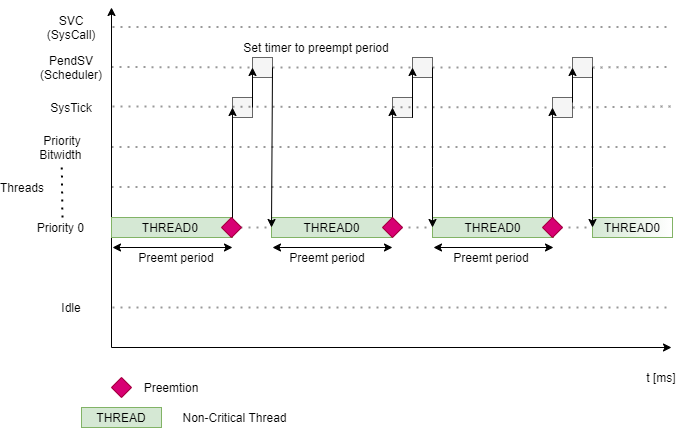
\includegraphics[width=1\textwidth]{images/performance_scheduling.png}
\caption{Performance scheduling diagram based only on preempt period}
\label{fig:PerformanceScheduling}
\end{center}
\end{figure}

\subsubsection{Hybrid scheduling}
As aforementioned, the hybrid scheduling algorithm consists of classic and performance scheduling. With this combination, it is possible to schedule critical tasks and non-critical threads within one system. \\
\indent Figure \ref{fig:HybridScheduling} shows a hybrid scheduling diagram with naming conventions related to the reference hardware architecture.\\
\indent The main characteristics of the hybrid scheduling algorithm are:
\begin{itemize}
\vspace{-0.2cm}\item Tasks are periodically scheduled and cannot be preempted, but just terminated.
\vspace{-0.2cm}\item Threads are scheduled based on their unique priority and can be preempted when one of the mentioned events (\ref{performanceSchedulingSubSubsection}) occurs.
\end{itemize}

\begin{figure}[H]
\begin{center}
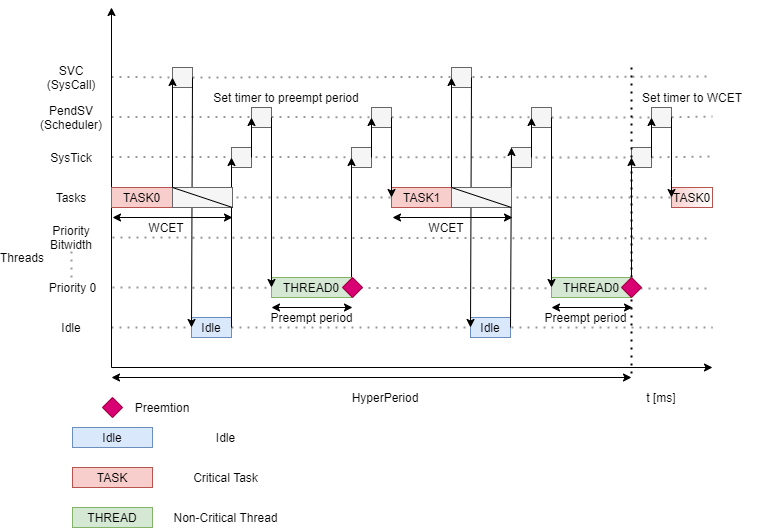
\includegraphics[width=1\textwidth]{images/hybrid_scheduling.png}
\caption{Hybrid scheduling diagram}
\label{fig:HybridScheduling}
\end{center}
\end{figure}

\subsubsection{Thread sleep}
Thread sleep implemented in CosmOS is used for suspending thread execution for the required periods of time. For this purpose, every thread has its alarm with timer and state variable configured in the operating system, as it was mentioned before in subsection \ref{alarm}. The internal alarm timer has the same period as the scheduler preempt period. Still, we are not interrupting the task for the specified worst-case critical execution time during the critical task execution. However, the timer won't be updated for this period. Inaccuracy can also be caused by executing a higher priority thread, which can delay the execution of the unblocked thread with an expired alarm. \\
\indent Figure \ref{fig:exactSleepTime} shows the most accurate result that can be achieved with thread sleep. The thread sleep \ac{API} is called before the system timer interrupt occurs. The required sleep period is 1 ms which is the same as the preemption period. During the sleep state of thread 0, thread 1 with higher priority is executed, but afterward, it's blocked (e.g., by unsuccessful mutex locking) before the system timer interrupt occurs. The thread 0 alarm is updated during the scheduler execution triggered by the system timer. As the alarm expires for thread 0, it can be set to the ready state, and as there is no higher priority thread ready, it can be scheduled again.
\begin{figure}[H]
\begin{center}
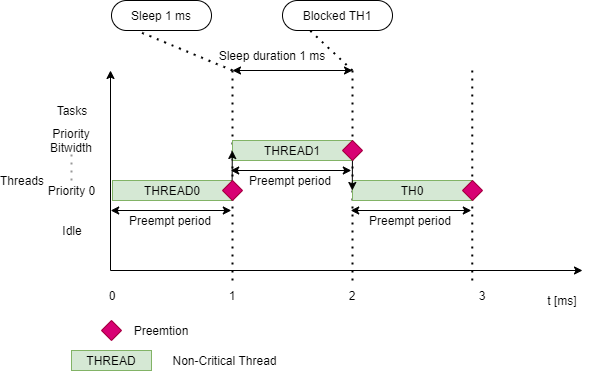
\includegraphics[width=1\textwidth]{images/thread_sleep_exact.png}
\caption{Exact sleep time}
\label{fig:exactSleepTime}
\end{center}
\end{figure}

Figure \ref{fig:threadExceedingSleep} shows an example of the inaccuracy of the thread sleep. The thread sleep \ac{API} is called in the middle of the preemption period. The required sleep period is 1 ms, which is the same as the preemption period. During the sleep state of thread 0, thread 1 with higher priority is executed, but afterward, it is preempted by the system timer interrupt, and the scheduling algorithm is called. The scheduling algorithm picks the critical task as its start time, and the system timer is set to the \ac{WCET}. The thread 0 alarm is updated during the scheduler execution triggered by the system timer after the \ac{WCET}. As the alarm expires for thread 0, it can be set to state ready and scheduled again, but thread 1 is still in state ready. Therefore, the scheduling algorithm picks it again. After some point, thread 1 is blocked (for instance, by unsuccessful mutex locking), and as there is no higher priority thread waiting, thread 0 can be scheduled again.
\begin{figure}[H]
\begin{center}
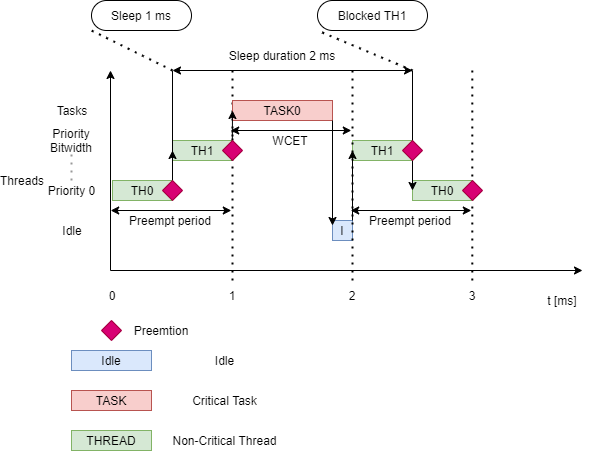
\includegraphics[width=1\textwidth]{images/thread_sleep_longer.png}
\caption{Exceeding the required sleep time}
\label{fig:threadExceedingSleep}
\end{center}
\end{figure}

\subsection{System jobs}
The system jobs module allows the user to run critical software (e. g. drivers) in the kernel space. \\
\indent This module reduces otherwise necessary system calls from the user space and decreases the execution time of the critical software.\\
\indent All system job handlers (classic c language non-returning functions) run under critical tasks and inherit all critical task properties. Still, it is possible to create an inner period for each group of handlers within this task. The system jobs group period is based on the system job task period. It can be multiplied by the group period multiplier to increase the inner period for a specific system job group when it does not have to be scheduled every time the system jobs task is scheduled, as is shown in figure \ref{fig:SysJobsScheduling}. The system jobs group G0 in figure \ref{fig:SysJobsScheduling} is scheduled every time the system jobs task runs, but the system jobs group G1 is scheduled every second time as it uses the inner scheduling feature of the system jobs group.

\begin{figure}[H]
\begin{center}
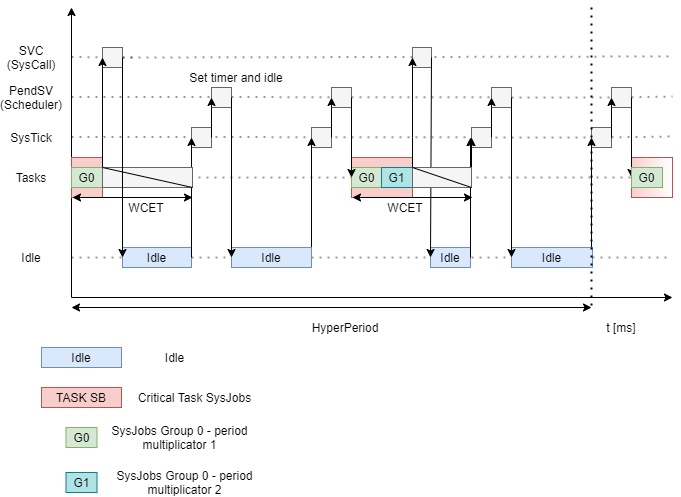
\includegraphics[width=1\textwidth]{images/sys_jobs_scheduling.png}
\caption{System jobs inner scheduling example}
\label{fig:SysJobsScheduling}
\end{center}
\end{figure}

The main characteristics of the system jobs group are shown in table \ref{tab:SysJobsGroupFeatures}.

\begin{table}[H]
\centering
\caption{ System Jobs Group main characteristics }
\centering
\begin{tabular}{|c|c|}
\hline
& \textbf{System Job Group} \\
\hline \hline
Is periodic with task period\cdot multiplier & \checkmark \\
\hline
Can be preempted & --- \\
\hline
Is killed after \ac{WCET} & \checkmark \\
\hline
Stack space is reused & \checkmark \\
\hline
Floating-point usage allowed & \checkmark\\
\hline
Can use dynamic allocation & --- \\
\hline
Can use spinlocks & \checkmark \\
\hline
Can use mutexes & ---  \\
\hline
Can use semaphores & ---  \\
\hline
Can use buffers (inter-program, inter-core) & \checkmark \\
\hline
Can use channels (inter-program, inter-core) & --- \\
\hline
Can handle interrupts & --- \\
\hline
Can be put to sleep & --- \\
\hline
\end{tabular}
\label{tab:SysJobsGroupFeatures}
\end{table}


\subsection{Core}
The core module is mainly used as a configuration module that contains all necessary information about configured cores in the operating system. The core module is an abstraction for the specific \ac{CPU} and is assigned via the CosmOS CustomBox \ac{GUI}. Cores collect programs specifically bound to them. Users can easily assign a specific program to the desired core to access to specific \ac{CPU} resources. The core also has its memory sections for the user, unmapped code executed by it, and unmapped data (static and variable) described in subsection \ref{memoryMapping}. These core-specific memory sections can be configured via the CosmOS CustomBox \ac{GUI} in the tab Cores. The simplified diagram of the core structure is shown in figure \ref{fig:coreStructure}.

\begin{figure}[H]
\begin{center}

\includegraphics[width=0.5\textwidth]{images/core_structure.png}
\caption{Core structure simplified diagram}
\label{fig:coreStructure}
\end{center}
\end{figure}

\subsection{Permission}\label{Permission}
The permission module enables the user to protect specific system resources such as buffers.\\
\indent It is possible to configure permissions for read/write access to some resources.
The implementation of the permissions strives to find a golden mean between memory consumption and execution time. Therefore, the information about access permission for specific schedulable is stored as bit, and we can evaluate it with fast bit-shift operations.\\
\indent To enhance the security of the permissions module, the inverted values are generated and stored in memory to ensure that no data is corrupted during the runtime, as is shown in figure \ref{fig:Permissions}.


\begin{figure}[H]
\begin{center}
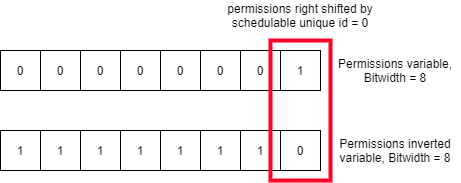
\includegraphics[width=0.8\textwidth]{images/permissions.png}
\caption{Permission variables example}
\label{fig:Permissions}
\end{center}
\end{figure}

\subsection{Buffer}
The buffer module is part of the CosmOS data exchange interface. It is mainly used for inter-program critical tasks communication but not constrained to that. Threads can also use buffer interface but we strongly suggest to use channels to increase overall performance of the system.

\paragraph{Buffer}\mbox{}\\
\indent Buffer unit implements the circular buffer logic adjusted to be used in the operating system. 
Buffer storage areas are mapped to the operating system memory. Specifically, \ac{OS} variables are described in detail in paragraph \ref{osSections}. As this memory section can be accessed only by privileged software, the user can not access the buffers from the user space directly. Besides the classic memory protection against unprivileged read/write operations, the buffers also use the permission module, which can restrict the buffer read/write access to the schedulable tasks/threads. These access permissions are checked when the buffer read/write \ac{API} is called by the task/thread. The size of the buffer storage areas, together with the permissions, can be configured via the CosmOS CustomBox \ac{GUI} in the tab Buffers. Data coherency for the buffer read/write operations in the multi-core environment is achieved within the \ac{API} that uses synchronization primitives (spinlocks) internally during each requested read/write operation. Therefore we suggest to to use a buffer interface for the critical tasks as they can not be preempted. The simplified diagram of the buffer structure is shown in figure \ref{fig:bufferStructure}.
\begin{figure}[H]
\begin{center}

\includegraphics[width=0.55\textwidth]{images/buffer_structure.png}
\caption{Buffer structure simplified diagram}
\label{fig:bufferStructure}
\end{center}
\end{figure}

\paragraph{Double buffer}\mbox{}\\
\indent The double buffers are an extension built on the top of the classic buffers and inherit all their properties. Upon them, we implemented a logic to differentiate which kernel occupies buffer from the buffer pair (two classic buffers) and which by the user. The simplified diagram of the double buffer structure is shown in figure \ref{fig:doubleBufferStructure}.

\begin{figure}[H]
\begin{center}

\includegraphics[width=0.55\textwidth]{images/doubleBuffer_structure.png}
\caption{Double buffer structure simplified diagram}
\label{fig:doubleBufferStructure}
\end{center}
\end{figure}

\subsection{Channel}
The channel module is part of the CosmOS data exchange interface. It can only be used for inter-program thread communication.\\
\indent Channels use specific memory areas to transfer data between the sender and receiver called pools. \\
\indent Each channel pool is placed in the operating system memory section. Specifically, \ac{OS} variables are described in detail in paragraph \ref{osSections}. As this memory section can be accessed only by privileged software, the user can not access the channel pool from the user space directly. Besides the classic memory protection against unprivileged read/write operations, the channels also use the permission module, which restricts the channel send/reply access to the specific threads. These access permissions are checked when the channel send/reply \ac{API} is called by the thread. The size of the channel pools, together with the permissions, can be configured via the CosmOS CustomBox \ac{GUI} in the tab Channels. Data coherency for the channel send/reply operations in the multi-core environment is achieved within the \ac{API} that uses synchronization primitives (semaphores) internally during each requested send/reply operation. This constrains the usage of the channels to the thread type of schedulables.
The simplified diagram of the channel structure is shown in figure \ref{fig:channelStructure}.
\begin{figure}[H]
\begin{center}

\includegraphics[width=0.55\textwidth]{images/channel_structure.png}
\caption{Channel structure simplified diagram}
\label{fig:channelStructure}
\end{center}
\end{figure}

\indent The simplified concept of the channel is the interface for the synchronized data transfer between sender (can be imagined as a client) and reply (can be imagined as a server) thread. Channel implementation currently supports data transfer from multiple sender threads to one reply thread. \\
\indent In the figure \ref{fig:channel} is shown the reply thread receive loop on the right side, where the thread signalizes first all the clients with the channel receive function call that is ready to receive data and if there is no data available the reply thread is put to the listening state and subsequently blocked by the scheduler. \\ 
\indent On the left side of figure \ref{fig:channel} the sender thread is shown. It requests data transfer by calling the channel send function and also signalizes the channel interface that it expects reply by calling the channel send function with a non-zero local reply pool size. Therefore the sender thread is put into the state waiting for reply and blocked by the scheduler till the reply occurs. Channel send function signalizes the reply thread that the data are available and if it is blocked by running (in state listening), the state is again set to ready, and reschedule triggered if the thread in execution priority is less than the reply thread priority. The reply thread is scheduled again and can process the data from the sender thread. Afterward the reply thread calls channel reply function to transfer the reply to the sender if the sender is waiting for the reply. In that case, the sender thread is signalized, its state is again set to ready, and reschedule triggered if the thread in execution priority is less than the sender thread priority. The sender thread can now process the reply.
\begin{figure}[H]
\begin{center}
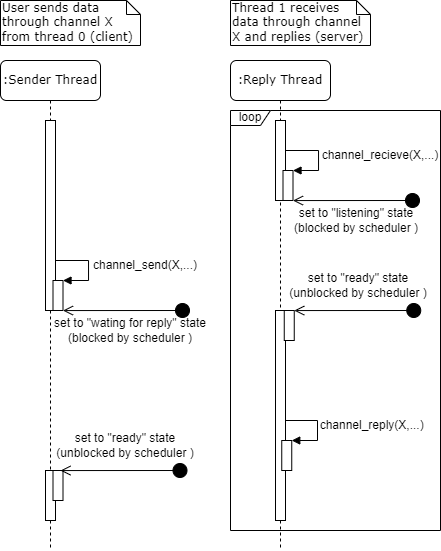
\includegraphics[width=0.7\textwidth]{images/channel.png}
\caption{Data exchange via channel sequence}
\label{fig:channel}
\end{center}
\end{figure}

\subsection{System calls}
The system calls module is used as an interface for transporting a specific number of arguments (with specified type) to the system call dispatcher, which uses the route module to retrieve the correct function, as is explained in subsection \ref{Route}.

\subsection{Route}\label{Route}
The route module is dedicated to mapping system calls to specific function handlers and entities.\\
Currently, the system calls are used as an interface function for passing correct arguments types. This allows us to have mapped multiple function handlers and entities to the one system call interface function. To achieve such behavior, we need to have a unique route identifier and retrieve the correct function and entity in the system call dispatcher. Routes can be configured via the CosmOS CustomBox \ac{GUI} in the tab Routes by the user or system integrator if there is a need to add some specific kernel side service.

\begin{figure}[H]
\begin{center}
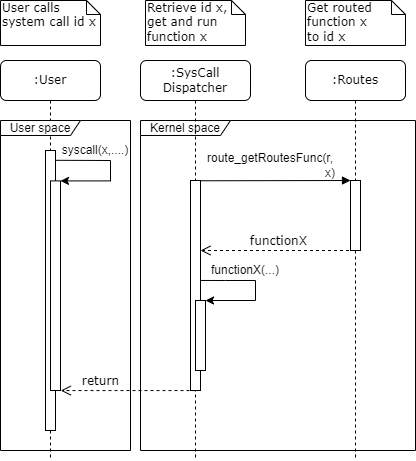
\includegraphics[width=0.65\textwidth]{images/routes_example.png}
\caption{System call sequence}
\label{fig:SysCallDispatcher}
\end{center}
\end{figure}

\subsection{OS}
The OS module is mainly used as a configuration module that contains all necessary information about the operating system and provides \ac{API} for interacting with the operating system structure. The operating system structure is an abstraction structure that stores all configured system structures, such as cores and channels, etc. The operating system structure must be available across all \ac{MCU} masters. The simplified diagram of the operating system structure is shown in figure \ref{fig:osStructure}. Besides the interaction with the operating system structure, the operating system module contains multiple units such as initialization, boot, or events unit.

\begin{figure}[H]
\begin{center}

\includegraphics[width=0.55\textwidth]{images/os_structure.png}
\caption{Operating system structure simplified diagram}
\label{fig:osStructure}
\end{center}
\end{figure}

\subsection{Boot}
The operating system boot unit is used mainly for the boot and validation of the configured memory section in the operating system. \\
\indent The boot sequence implements copy and set memory operations for the loading configured sections into the volatile from the non-volatile memory or setting the uninitialized data memory sections to zero. \\
\indent It is highly suggested to call the boot sequence right after the \ac{MCU} start-up. \\
\indent After the boot is finished we are able to proceed with the operating system initialization.

\subsection{Initialization}
The operating system initialization unit prepares the hardware for the operating system start-up and initializes all operating system modules, such as a memory protection unit or memory manager unit. \\
\indent The initialization sequence takes place after the operating system boot sequence and user-specific hardware configuration. After the initialization of the hardware and all modules, the validation of the boot and initialized modules is performed.\\
\indent The initialization must be finished before the operating system is started.

\subsection{Event}
The operating system event unit handles the triggering and dispatching of the events within the operating system. \\
\indent The main idea of the operating system events is to be able to trigger event from one core and handle it with the others. On the left side of figure \ref{fig:osEvent} the event trigger mechanism is shown. The core with identifier 0 triggers the event X on the core with identifier 1. It is also possible to choose just some of the cores in a multi-core system. After the event is triggered, the hardware mechanism present on the \ac{MCU} must signalize the other core. In our example it is the core with the identifier 1. On this specific core the handler function for the event X is dispatched by the operating system dispatch function. After the event handler function was dispatched, the core signalizes all cores that a new event can be triggered in the operating system again.
\begin{figure}[H]
\begin{center}
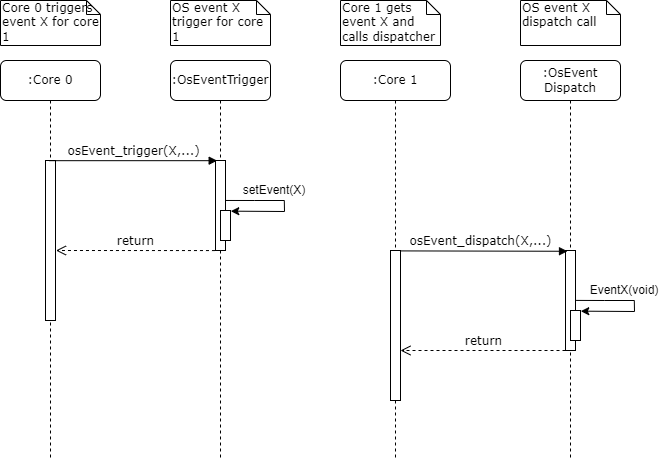
\includegraphics[width=1\textwidth]{images/events_example.png}
\caption{Operating system event call}
\label{fig:osEvent}
\end{center}
\end{figure}
Events use specific memory areas to transfer data between the core that triggers the event and the core that handles it. \\
\indent The event pool is placed in the operating system memory section. Specifically, \ac{OS} variables are described in detail in paragraph \ref{osSections}. As this memory section can be accessed only by privileged software, the user can not access the event pool from the user space directly.\\
\indent Events also use a generic mapping mechanism of the event handler functions based on the event identifiers. With this approach, it is possible to configure the event unit via the CosmOS CustomBox \ac{GUI} in the tab Events by the system integrator if there is a need to add some specific operating system event.

\subsection{Memory}
The memory module consists of three units: memory mapping, protection, and manager.
\subsubsection{Memory mapping}\label{memoryMapping}
The memory mapping unit is dedicated to mapping all application, core, and in- integration layer sections to the physical memories. For this purpose, memory mapping macros and the linker scripts are generated to ease the mapping of all sections.

\paragraph{Stack section}\mbox{}\\
\indent CosmOS consists of three types of stack memory sections: kernel, task, and thread. All stacks are contiguous memory sections in physical memory with some minor differences in the mapping and re-usability.\\
\indent The low address of all types of the stacks memory section is aligned based on the selected \ac{MCU} architecture. \\

\textbf{Kernel} stack section: mapped to the configured physical memory by the system integrator, as is shown in figure \ref{fig:StacksMapping}. The size of the kernel stack can be configured in the CosmOS CustomBox.\\

\textbf{Task} stack section: mapped to the configured physical memory by the system integrator, as is shown in figure \ref{fig:StacksMapping}. The task stack size is the biggest stack size of all tasks attached to the current core.\\
\indent The task in execution always reuses the stack memory because a task cannot be preempted.\\

\textbf{Thread} stack section: mapped to the configured physical memory by the system integrator, as is shown in figure \ref{fig:StacksMapping}.\\
\indent The size of the thread stack can be configured in the CosmOS CustomBox for each thread separately.

\begin{figure}[H]
\begin{center}
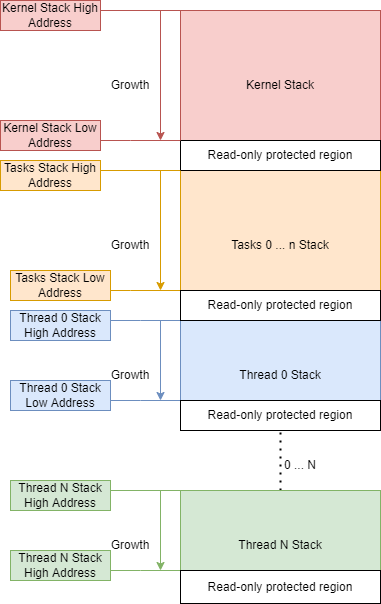
\includegraphics[width=0.6\textwidth]{images/stacks_mapping.png}
\caption{Stacks memory sections layout}
\label{fig:StacksMapping}
\end{center}
\end{figure}

\paragraph{Program section}\label{programMemorySection}\mbox{}\\
\indent The program memory section contains the heap and data subsections, and is a contiguous block mapped to the configured physical memory. The program data subsection is divided into the initialized and uninitialized data, and its size can be configured in the CosmOS CustomBox.\\
\indent The low address of this memory section is aligned based on the selected \ac{MCU} architecture. \\

\textbf{Heap} is a subsection on top of the program memory layout, as is shown in figure \ref{fig:ProgramMapping}.\\
\indent The size of the program heap can be configured in the CosmOS CustomBox for each program separately.\\

\textbf{Initialized data} is a subsection of the program memory layout, as is shown in figure \ref{fig:ProgramMapping}.\\
\indent The initialized data subsection contains all initialized data belonging to the current program.\\

\textbf{Uninitialized data} is a subsection of the program memory layout, as is shown in figure \ref{fig:ProgramMapping}.\\
\indent The uninitialized data subsection contains all uninitialized data belonging to the current program.

\begin{figure}[H]
\begin{center}
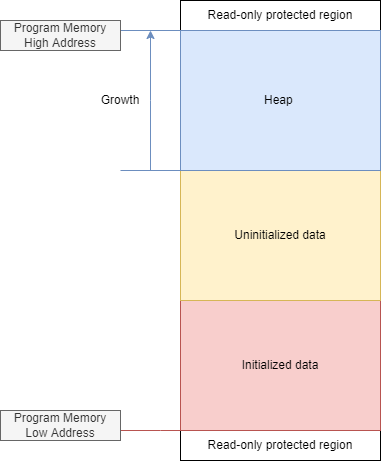
\includegraphics[width=0.6\textwidth]{images/program_mapping.png}
\caption{Program memory section layout}
\label{fig:ProgramMapping}
\end{center}
\end{figure}

\paragraph{OS section}\label{osSections}\mbox{}\\
\indent CosmOS consists of the three types of \ac{OS} sections: constant, variable, and functions. All types of \ac{OS} sections are contiguous memory sections in physical memory.\\
\indent In multicore systems, all \ac{OS} sections have to be mapped by the system integrator to physical memory shared between all cores.\\
\indent The low address of all types of the \ac{OS} sections is aligned based on the selected \ac{MCU} architecture. \\

\textbf{Constant} is a section for constant system data - they stay constant during the runtime. The size of this section can be configured in the CosmOS CustomBox.\\
\indent This memory section can be cached for improving performance since it contains only constant data, and thus, no cache invalidation during runtime is needed. \\

\textbf{Variable} is a section for variable system data - they do not have to stay constant during the runtime. The size of this section can be configured in the CosmOS CustomBox.\\
\indent This memory section can be cached, but cache invalidation must be performed every time the data changes.\\

\textbf{Function} is a section for system functions. The size of this section can be configured in the CosmOS CustomBox.\\
\indent This memory section can be cached for improving performance since it contains only code, and thus, no cache invalidation during runtime is needed.

\paragraph{User code section}\label{userCodeMemoryMapping}\mbox{}\\
\indent User code is a section for user functions such as task/thread handlers or any support program functions appropriately mapped to that specific program. The size of this section can be configured in the CosmOS CustomBox.\\
\indent This memory section can be cached for improving performance since it contains only code, and thus, no cache invalidation during runtime is needed.\\
\indent The low address of this memory section is aligned based on the selected \ac{MCU} architecture.

\paragraph{Unmapped static data section}\label{staticDataMemoryMapping}\mbox{}\\
\indent The unmapped static data section is a contiguous block of memory-mapped to the configured physical memory, and its size can be configured in the CosmOS CustomBox.\\
This section contains all static data (declared by users and also libraries).\\
\indent This memory section can be cached for improving performance since it contains only constant data, and thus, no cache invalidation during runtime is needed. \\
\indent The low address of this memory section is aligned based on the selected \ac{MCU} architecture.

\paragraph{Unmapped variable data section}\mbox{}\\
\indent The unmapped variable data section is a contiguous block of memory-mapped to the configured physical memory, and its size can be configured in the CosmOS CustomBox.\\
This section contains all variable data (e. g., variables from libraries) and the heap section for libraries or dynamic allocations before the operating system starts up, as shown in figure \ref{fig:UnmappedDataSection}.\\
\indent The low address of this memory section is aligned based on the selected \ac{MCU} architecture.

\begin{figure}[H]
\begin{center}
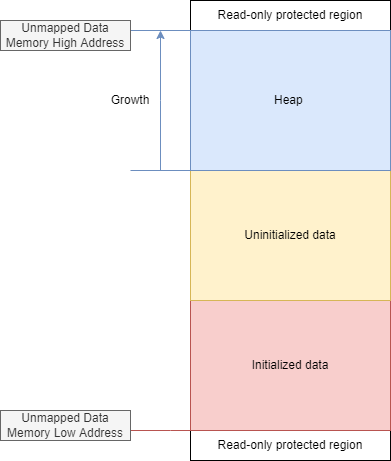
\includegraphics[width=0.6\textwidth]{images/unmapped_data.png}
\caption{Unmapped data memory section layout}
\label{fig:UnmappedDataSection}
\end{center}
\end{figure}

\paragraph{Unmapped code section}\mbox{}\\
\indent The unmapped code section is a contiguous block of memory-mapped to the configured physical memory, and its size can be configured in the CosmOS CustomBox.\\
This section contains all unmapped code (e.g., code from libraries).\\
\indent The low address of this memory section is aligned based on the selected \ac{MCU} architecture.

\subsubsection{Memory protection}

The memory protection software unit is dedicated to reconfiguring the memory protection regions either during initialization or runtime of the operating system. This is an optional feature and can be deactivated with the switch module (\ref{switchModule}).

\paragraph{Stack section}\mbox{}\\
\indent The memory protection software unit is used for task/thread protected memory region operating system runtime reconfiguration and kernel stack configuration during operating system initialization.\\
\indent Task/thread stack protected memory regions are reconfigured when executing the scheduler algorithm for the task/thread that will be executed next.  Read-write operations can access it by unprivileged and privileged software.  The task/thread stack protected memory region from the prior execution is reconfigured back to its no-access protected memory region.\\
\indent Stack overflow protection is achieved with a small no-access protected memory region in the stack growth direction.\\

\textbf{Kernel} stack section: This protected memory region can be accessed for write operations only by privileged software. Unprivileged software can only read from this memory region.\\

\textbf{Task} stack section: This protected memory region can be accessed for read-write operations by unprivileged and privileged software only when the task is currently in execution; otherwise, the task stack is a no-access protected memory region.\\

\textbf{Thread} stack section: This protected memory region can be accessed for read/write operations by unprivileged and privileged software only when the thread is currently executed; otherwise, the thread stack is a no-access protected memory region.

\paragraph{Program section}\mbox{}\\
\indent The program-protected memory region is reconfigured during the execution of the scheduler algorithm for the program. Unprivileged and privileged software can access it for read-write operations. The program-protected memory region from a prior execution is reconfigured back to a no-access protected memory region. Program-protected memory regions can be accessed only by the tasks and threads bound to that specific program.\\

\paragraph{OS section}\label{programMemoryProtection}\mbox{}\\
\indent OS-protected memory regions (constant, variable, and function) are configured during the operating system initialization.\\

\textbf{Constant} section: Privileged and unprivileged software can access a protected memory region for only read operations.\\

\textbf{Variable} section: Privileged software can access a protected memory region for only write operations. Unprivileged software can only read from this memory region.\\

\textbf{Function} section: Privileged and unprivileged software can access a protected memory region for only read operations.

\paragraph{User code section}\label{userCodeMemoryProtection}\mbox{}\\
\indent Privileged and unprivileged software can access a protected memory region for only read operations.

\paragraph{Unmapped static data section}\label{userStaticDataMemoryProtection}\mbox{}\\
\indent Privileged and unprivileged software can access a protected memory region for only read operations.

\paragraph{Unmapped variable data section}\mbox{}\\
\indent Privileged and unprivileged software can access a protected memory region for read-write operations.

\paragraph{Unmapped code section}\label{unmappedCodeParagraph}\mbox{}\\
\indent Privileged and unprivileged software can access a protected memory region for only read operations.

\paragraph{Peripheral access section}\mbox{}\\
\indent For accessing \ac{MCU} peripherals directly from task/thread and not via a system call, we need to configure a low address and size in a specific task/thread peripheral to create a temporary protected memory region (figure \ref{fig:PeripheralAccess}). It will be reconfigured during the scheduling algorithm execution for unprivileged software read-write operations for the specific task/thread.

\begin{figure}[H]
\begin{center}
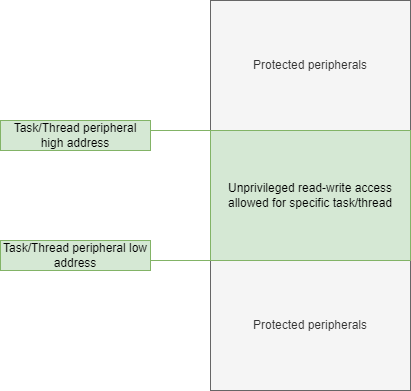
\includegraphics[width=0.6\textwidth]{images/peripheral_access.png}
\caption{Accessing specific peripherals from task/thread}
\label{fig:PeripheralAccess}
\end{center}
\end{figure}

\subsubsection{Memory manager}
This software unit is used for initializing and managing program heap and stack memory sections.\\
\indent Dynamic memory allocation and deallocation functions used in the C++ new/delete operators used after operating system start-up are implemented within the support CosmOS standard library. These support malloc and free functions use standard kernel modules \ac{API} interfaces to get the necessary information about the program in execution and its heap. Heap memory for each program has its mutex generated by the \ac{OS} for a specific program data memory for the allocation and de-allocation operations.

\paragraph{Dynamic allocations}\mbox{}\\
\indent \textbf{New operator}: Implemented within the CosmOS Support module. This implementation is not restricted to use only during the operating system run-time. For the correct function of the new operator before operating system start-up, the heap memory is allocated within the unprotected data memory section, as was mentioned in paragraph \ref{unmappedCodeParagraph}.\\
\indent During the operating system runtime, the support CosmOS standard library malloc function is called.\\

\textbf{Delete operator}: Implemented within the CosmOS Support module. This implementation is not restricted to use only during the operating system run-time. For the correct function of the new operator before the operating system start-up, the heap memory is allocated within the unprotected data memory section, as was mentioned in paragraph \ref{unmappedCodeParagraph}.\\
\indent During the operating system runtime, the support CosmOS standard library free function is called.\\

\textbf{Support malloc}: This function allocates memory for threads running in the CosmOS application layer. This function can be used only during the operating system run-time. The heap in each program must be initialized with the malloc variable placed at the heap memory low address, which is done during the operating system initialization.\\
\indent The function places a malloc variable on the heap during every allocation. It is linked with all variables currently allocated in a specific program heap in a linked list. The allocated memory chunk is placed above the aligned malloc variable, as is shown in figure \ref{fig:HeapAllocation}.\\

\textbf{Support free}: This function implementation is used to free memory for the threads running in the CosmOS application layer. This function can be used only during the operating system run-time. The heap in each program must be initialized with the malloc variable placed at the heap memory low address, which is done during the operating system initialization.\\
\indent The function removes the malloc variable from the linked list of all variables currently allocated in a specific program heap during each free operation.

\begin{figure}[H]
\begin{center}
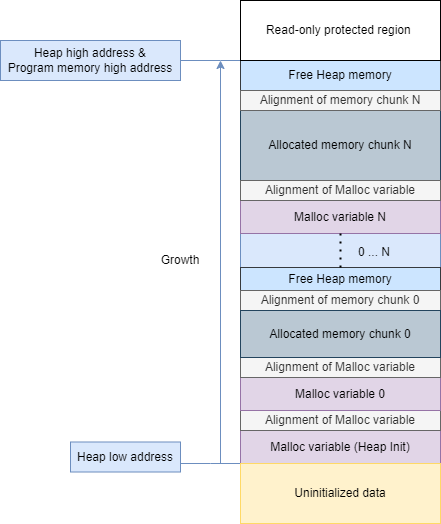
\includegraphics[width=0.6\textwidth]{images/heap_allocations.png}
\caption{Dynamic memory allocation layout}
\label{fig:HeapAllocation}
\end{center}
\end{figure}

\subsection{Interrupt}
The interrupt module is dedicated to configure and dispatch all interrupts in the system. In the CosmOS, we differentiate between two types of interrupts handling techniques - fast
and slow. \\

\textbf{The fast} interrupt is a method where the interrupt is handled directly in the \ac{ISR} as it is shown in the figure \ref{fig:fastInterrupts}. This allows users to handle the most critical interrupts immediately, and it the interrupt service routine execution time should be very low.

\begin{figure}[H]
\begin{center}
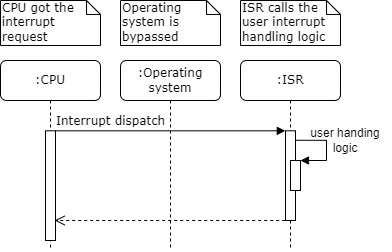
\includegraphics[width=0.55\textwidth]{images/fast_interrupt.png}
\caption{Fast interrupt sequence}
\label{fig:fastInterrupts}
\end{center}
\end{figure}

\textbf{The slow} interrupt is a method where the interrupt is handled in its specific thread as it is shown in the figure \ref{fig:slowInterrupts}. The thread is unblocked after the interrupt occurs and blocked again when it is handled. This allows users to create non-blocking interrupt handling directly in the user space for non-critical interrupts and therefore it is possible to implement much more complex algorithms inside the handling thread. We still suggest keeping the handler thread algorithm complexity at the minimum.

\begin{figure}[H]
\begin{center}
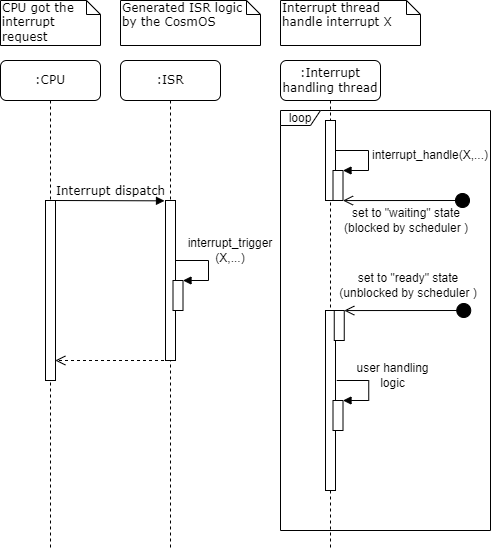
\includegraphics[width=0.8\textwidth]{images/slow_interrupt.png}
\caption{Slow interrupt sequence}
\label{fig:slowInterrupts}
\end{center}
\end{figure}

\subsection{Error handler}
The error handler module detects, traces, and handles all errors which can occur within the operating system. \\
\indent The errors are traced for every program configured in the operating system that can be later used for the debug purpose. Error processing allows triggering the required error reaction, which can be configured in the CosmOS CustomBox.

\subsection{API}
CosmOS API module is an interface module with a set of provided \ac{API} to ease the interaction between the user and the operating system core modules, as is shown in figure \ref{fig:CosmOSAPI}.

\begin{figure}[H]
\begin{center}
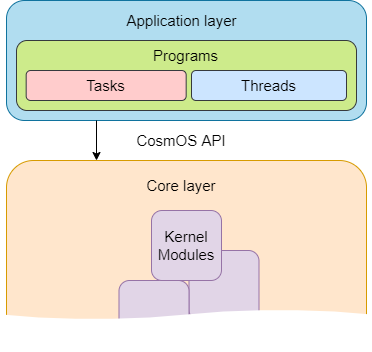
\includegraphics[width=0.5\textwidth]{images/cosmos_api.png}
\caption{CosmOS API layers connection}
\label{fig:CosmOSAPI}
\end{center}
\end{figure}

\ac{API} provides functions like macro, and it interfaces with a pre-generated system call route identifier for the routes configured via the CosmOS CustomBox.\\
\indent Figure \ref{fig:CosmOSAPIfunctionAsMacro} shows how the function like macro is generated. The name of the function is generated based on the routes configuration in the CosmOS CustomBox. The used type of the system call is also generated based on the configuration of the specific route together with the return type and function arguments. The system call identifier is generated number used during the dispatching of the system call handler function. It is mapped to the handler function configured in the route.

\begin{figure}[H]
\begin{center}
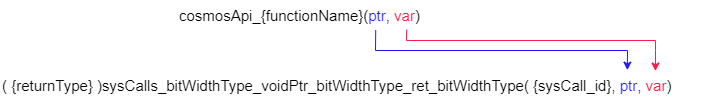
\includegraphics[width=1\textwidth]{images/cosmosAPI.png}
\caption{CosmOS generated function like macro API}
\label{fig:CosmOSAPIfunctionAsMacro}
\end{center}
\end{figure}


\section{Integration layer}
The integration layer is a type of microcontroller abstraction layer. The \ac{CIL} provides a set of \ac{API} required by the CosmOS core layer, as is shown in figure \ref{fig:CIL}.

\begin{figure}[H]
\begin{center}
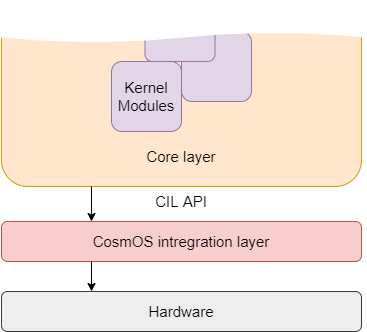
\includegraphics[width=0.5\textwidth]{images/cosmos_integration.png}
\caption{CosmOS integration layer}
\label{fig:CIL}
\end{center}
\end{figure}


\section{Application layer}
The CosmOS application layer is an abstraction layer where the user software is implemented. User software in this layer is running in unprivileged mode. Therefore, it is necessary to use the CosmOS API to interact with the kernel modules. The application layer consists of programs,  threads, and tasks, but sometimes in rare cases, it can also contain some handlers called in operating system hooks. In the C/C++ language terminology, the application layer consists of the generated source and header file pairs representing programs. Tasks, threads, or hooks are represented as function handlers with configured names of the task, threads, or hooks via the CosmOS CustomBox. Comments encapsulating parts that the user can change and are not deleted during the re-generation of the programs are placed in the program source files.

\subsection{Programs}
A program in the application layer can be represented, as mentioned before, as a source and header file. For each program, the necessary memory mapping macros are generated. Their usage is explained directly in the generated file to achieve data mapping to the specific program sections, such as initialized or non initialized data.
\subsubsection{Tasks}
Tasks are in the application layer and can be represented, as mentioned before, as a function handler. These functions are declared inside the schedulable kernel module but exposed during the linking phase. Each task code is automatically mapped to the specific application section and does not have to be explicitly mapped to program data by the user. The tasks are generated with all necessary information (e.g., \ac{WCET} or task period) to ease the implementation phase.
\subsubsection{Threads}
As mentioned before, threads are in the application layer and can be represented as a function handler. These functions are declared inside the schedulable kernel module but exposed during the linking phase. Each thread code is automatically mapped to the specific application section and does not have to be explicitly mapped to program data by the user.
\subsection{Hooks}
As mentioned before, hooks are in the application layer and can be represented as a function handler. During their execution, these functions are called inside the operating system hooks and must be implemented carefully as they are handled as privileged software.
\section{CustomBox}
The CustomBox is the \ac{GUI} that comes as part of CosmOS, and it is used to configure everything changeable in the system. The \ac{UI} is a generalized skeleton, which will dynamically adjust depending on the configuration input.
\paragraph*{} The idea behind this was to have a generalized \ac{UI} that can easily and quickly adopt new features. Adding a feature should require only minimal effort and the only thing that has to be changed to add support are the configuration files.
\paragraph*{} The \ac{UI} connects to all parts of the python codebase and brings everything together. The \ac{UI} will use the config parser to load the configuration from the config files and allow the generator invocation with the click of a button.
\paragraph*{} All of it is implemented in python. The \ac{UI} is built using PySide6, but the \ac{UI} elements presented will be parsed from the config files dynamically, meaning that 
it should never be necessary to edit any python code to add a new configuration field.
\paragraph*{} In addition, all CosmOS CustomBox specific implementations are completely abstracted away from the \ac{UI} base (see figure \ref{fig:UI_architecture}). It can easily be reused for other projects if so desired.
\begin{figure}[H]
\begin{center}
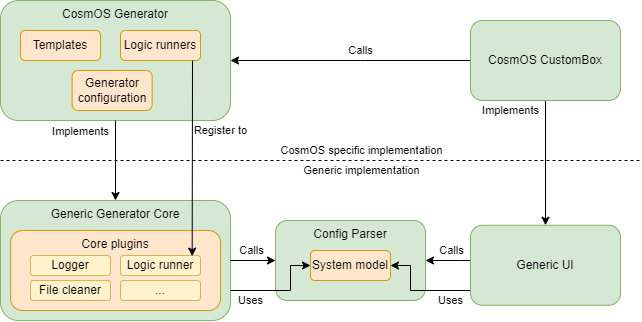
\includegraphics[width=1\textwidth]{images/custombox_architecture}
\caption{CosmOS CustomBox architecture}
\label{fig:UI_architecture}
\end{center}
\end{figure}

\subsection{Parser}

The parser used by both CustomBox and the config generator, as seen in figure \ref{fig:UI_architecture}, was built to be completely generic and reusable. Upon invocation, the parser will load all configuration files,  validate all defined values and do some processing on some of the more complex data types (we called it linking). In the end, it will provide one huge object, which we call the (system) model, containing all of the information from the config files in an easy-to-use way. This object provides a unified and generic \ac{API}, which will always stay the same no matter which data type a certain value is or how the config files' model configuration was set up. This \ac{API} is used every time any information is requested/changed.  All changes done through this \ac{API} will be validated against a basic set of rules defined in the config files before being saved to the model.
\paragraph*{} The model also provides member functions to check if the configuration was modified during runtime. It checks if it is different from the config files from which it was created. It also provides a function for serializing the current state of the object. That means that the model can serialize itself, but the parser is required for deserialization and will yield a new instance of the model object.
\paragraph*{} There are no warnings in any of the parser's code. Any misconfiguration, invalid value, wrong function call, or other errors will result in a python exception that we tried to make as helpful and descriptive as possible.

\subsubsection{Configuration}

One of the main goals was to create a simple-to-use configuration structure that can easily cover many different use cases while offering much flexibility to the user.
The main idea was to have a configuration that holds all of the following:
\begin{itemize}
\vspace{-0.2cm}\item the configured values
\vspace{-0.2cm}\item information about the datatypes of those values
\vspace{-0.2cm}\item the hierarchy of how elements relate to each other
\vspace{-0.2cm}\item the information about how to present all of this to a user in a nice looking graphical user interface
\end{itemize}

\paragraph*{} All of this configuration could be either done in one \ac{JSON} file containing every configuration parameter needed for the whole system or, like in our case, many different \ac{JSON} files in multiple subdirectories and even split across two repositories. A user setting up a new system would be completely free to choose the granularity to split up the configuration.

\paragraph{Terminology}\mbox{}\\
For a better understanding of how the structure is built up, refer to figure \ref{fig:config_structure} and the terminologies below:\\

\textbf{The Model}, also called
Configuration, is the data structure, or more specifically, the python class instance that contains all information from the config files. It contains one or more subconfigs, and the model also holds the attribute definition lookup table.\\

\textbf{A Subconfig} usually contains one or more elements, and it corresponds to one single \ac{JSON} file if that file contains any elements. A file that does not contain any elements will not get assigned to a subconfig.  A subconfig uses the name of the file it was loaded from, and its name must be unique. It is not supported that creating multiple config files with the same filename (which could be done because they could be in different subdirectories).\\

\textbf{An Element} is a single object that can hold one or more attributes, specifically, attribute instances. An element also has a name, which is used to access its attributes.\\

\textbf{An Attribute}, or more explicitly called Attribute  Instance,  is
the object that holds the actual value of some configuration parameter. An attribute instance has a name, an attribute definition, and a value.\\

\textbf{An Attribute Definition} is an object that holds all of the information about one particular attribute. An attribute definition could be reused for multiple attribute instances holding different information or belonging to different elements. An attribute definition will hold information about an attribute such as its type, validation information, label, and tooltips in the UI.\\



\begin{figure}[H]
\begin{center}
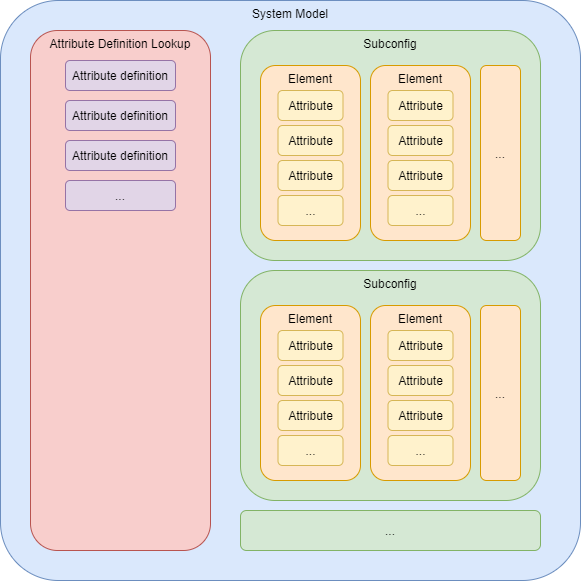
\includegraphics[width=0.8\textwidth]{images/parser_model_structure}
\caption{Configuration structure}
\label{fig:config_structure}
\end{center}
\end{figure}

\subsection{Generator}
The generator takes the configuration files together with some source and header file templates and a file generation config and creates source and header files from all of them. These source and header files are automatically generated correctly and will be considered during the next compilation of the CosmOS operating system. Upon invocation of the generator, it follows a specific sequence as in figure \ref{fig:generator_flow}

\begin{figure}[H]
\begin{center}
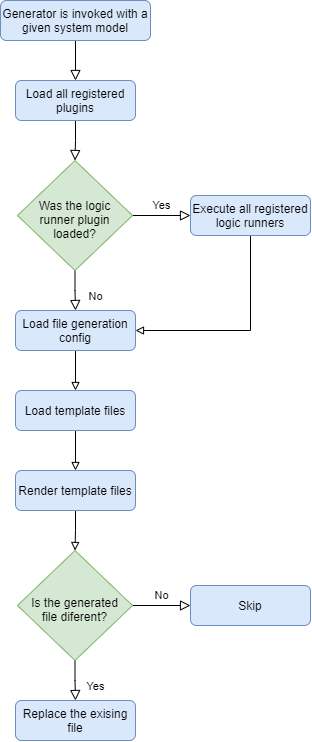
\includegraphics[width=0.4\textwidth]{images/generator_flow}
\caption{Generator sequence}
\label{fig:generator_flow}
\end{center}
\end{figure}

\subsubsection{Templates}
The templates are the heart of the generator. Additional logics, which could even be user-defined, are written into the templates. Templates are rendered using the python package jinja2, and the full feature set of that templating engine can be utilized. In the templates, users have full access to the whole system model and its \ac{API}. They can also access any needed data by using a nice syntax. For example: \inlinecode{model.cores.core0.coreId} would return the value of the \inlinecode{coreId} attribute instance of the element with the name \inlinecode{core0} defined in a subconfig named \inlinecode{cores}.

\subsubsection{File generation config}
The file generation configuration is needed for the generator to know where to find the template, which template should be rendered to which output file, and the way to do it. This part is kept generic. Only the configuration is CosmOS specific.


\subsection{Model}
Together with all its \textbf{logic runners}, the model creates an abstract representation of the operating system, which is used to generate files. The logic runners are small python plugins that are attached to the configuration generator. Logic runners use the system configuration files configured by the user via the CosmOS CustomBox \ac{GUI} for further module initialization or calculations, modifying parts of the model, filling in placeholder values, etc.

\subsubsection{Initializer}
The initializer logic runner initializes missing parameters in the model, such as unique and iterative identifier value assignments, to generate the module's configurations (e.g., in the arrays).

\subsubsection{Memory mapper}
The memory mapper logic runner is used to map all of the data sections mentioned in subsection \ref{memoryMapping}. The memory mapper does all necessary calculations for the alignment of the section sizes. The mapper also ensures low/high section addresses to be compatible with the memory protection unit for the specific architecture configured via the CosmOS CustomBox in the \ac{MCU} tab.

\subsubsection{Permissioner}
The permissioner logic runner compresses the permissions configured for the buffers via CosmOS CustomBox in the Buffers tab. The permissions based on the unique identifier of the schedulable have to be compressed to bit values, as was explained in subsection \ref{Permission}

\subsubsection{Scheduler}
The scheduler logic runner generates schedule table entries and composes static schedule tables, which are used for the classic scheduling algorithm described in subsubsection \ref{classicScheduling}.


\newpage

\vspace*{-2.5cm}
\chapter{Discover more}
To learn more about the project, we provide a list of links in this section to help you get started:
\begin{itemize}
\vspace{-0.2cm}\item \href{https://cosmos-creators.github.io}{Wiki} is our main knowledge base. It will provide you with all the necessary information about the project. You will find how to use the operating system with many examples, how you can contribute to the project, what tools we use, and all other essential information. We highly recommend starting with this page to find everything from the overview to the in-depth technical details.
\vspace{-0.2cm}\item \href{https://github.com/CosmOS-Creators}{Github} organization contains all repositories and projects. If you want to contribute to or use our project, this is the right place where you can get the latest source codes, tools and check the current issues.
\vspace{-0.2cm}\item \href{https://www.youtube.com/channel/UCWSxT8kLvbVGm-9HlEyiRUg}{YouTube} channel helps users understand the basics of the operating system and provides them plenty of examples to show how to use provided features. 
\vspace{-0.2cm}\item \href{https://www.linkedin.com/company/cosmoscreators}{LinkedIn} and \href{https://twitter.com/cosmos_creators}{Twitter} will keep you posted about the upcoming features, releases, and events.
\vspace{-0.2cm}\item \href{https://discord.gg/XTabzYYVxS}{Discord} is our community communication channel. All people interested in the project are welcome to join.
\end{itemize}


\end{document}
